\documentclass[12pt,a4paper]{article}
\usepackage[utf8]{inputenc}
\usepackage[T2A]{fontenc}
\usepackage[ukrainian]{babel}
\usepackage{fancyvrb}
\usepackage{pdflscape}

\usepackage{amsmath} % у преамбулі
\usepackage{array, multirow}
\usepackage{hyperref} % <-- Обов’язково підключіть цей пакет
\usepackage{caption}
\usepackage{booktabs}
\usepackage{subcaption} % для підписів (а), (б)
\usepackage{breqn} % Пакет для автоматичного перенесення виразів
\usepackage{mathtools} % Для додаткових можливостей, наприклад, для створення кастомних конструкцій
\usepackage{makecell} % Для створення багаторядкових комірок у таблицях

\usepackage{xcolor}

\renewcommand{\thetable}{№\arabic{table}}
\captionsetup[table]{name=Таблиця}  % замість "Табл." буде "Таблиця"

\usepackage{graphicx} % <-- Для роботи з \includegraphics
\usepackage{geometry}
\geometry{
    left=2cm,
    right=2cm,
    top=2cm,
    bottom=2cm
}


\begin{document}

    \begin{titlepage}

        \thispagestyle{empty}
        \begin{center}
        \large
        Національний технічний університет України\\
        «Київський політехнічний інститут імені Ігоря Сікорського»\\[1em]
        Факультет інформатики та обчислювальної техніки\\
        Кафедра загальної фізики
        \end{center}

        \vfill

        \begin{center}
        \textbf{\LARGE Фізика}\\[2em]
        \textbf{\Large Лабораторна робота №3-3}\\
        «Вивчення дифракції Фраунгофера світла на щілині та дифракційній ґратці» 
        \end{center}

        \vfill

        \begin{flushright}
        Виконав: студент 1 курсу ФІОТ, гр. ІО-41\\
        \textit{Давидчук А. М.}\\
        Залікова книжка № 4106\\[1em]
        Перевірив: \textit{Колган В.\,В.}
        \end{flushright}

        \vfill

        \begin{center}
        Київ -- 2025
        \end{center}

    \end{titlepage}

    \setlength{\parindent}{0pt}

    \textbf{\underline{Тема:}} «Вивчення дифракції Фраунгофера світла на щілині та дифракційній ґратці».

    \vspace{1em}

    \textbf{\underline{Мета:}} експериментально вивчити залежність інтенсивності світла від
    кутів дифракції, визначити довжину хвилі випромінювання.

    \vspace{1.5em}

    \begin{center} \textbf{\Large Теоретичні відомості} \end{center}
    \setlength{\parindent}{1.5em}

    \begin{center} \textbf{Дифракція плоскої монохроматичної хвилі на щілині} \end{center}

    Якщо на довгу вузьку щілину нормально падає плоска монохроматична хвиля, то розподіл інтенсивності світла на екрані залежно від відстані до центра
    щілини задається функцією:

    \begin{equation}
        I(\varphi) = I_0 \left( \frac{\sin(\pi b \lambda^{-1} \sin \varphi)}{\pi b \lambda^{-1} \sin \varphi} \right)^2,
        \tag{3.1}
    \end{equation}

    графік якої представлений на рис. (3.1):

    \begin{figure}[!ht]

        \renewcommand{\thefigure}{3.\arabic{figure}} % робимо "3.1", "3.2" і т.д.

        \centering
        % Підставляєте потрібний шлях та розмір зображення:
        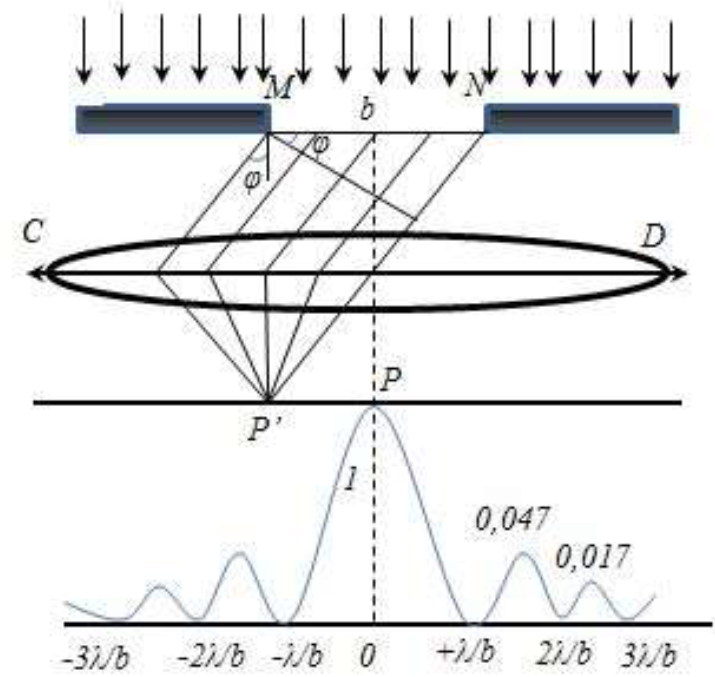
\includegraphics[width=0.3\textwidth]{3.1.png}
        % Підпис (зазвичай під малюнком):
        \caption{}
        % Мітка для посилань у тексті (\ref{fig:...})
        \label{fig1:schema}

    \end{figure}

    У формулі (3.1) $I_0$ --- інтенсивність хвилі, що падає, $\lambda$ --- довжина хвилі, $b$ --- ширина щілини.

    У розподілі можна виділити центральний максимум при $\varphi = 0$ та ряд побічних максимумів, напрямки на які залежно від кута $\varphi$ відхилення
    променів знаходиться за умовою:

    \begin{equation}
        b\varphi \approx \pm \left( 2n + 1 \right) \frac{\lambda}{2},
        \tag{3.2}
    \end{equation}

    де $n = 0, 1, 2, \dots$.
    Умова спостереження мінімумів, що розділяють максимуми:
    \[
    b\sin \varphi = \pm n \lambda,
    \]

    або для малих кутів:

    \begin{equation}
        b\varphi = \pm n \lambda.
        \tag{3.3}
    \end{equation}

    З умов екстремумів виходить, що зменшення ширини щілини призводить до
    збільшення відстані між мінімумами, тобто до розширення дифракційної
    картини.

    Якщо $b = \lambda$, то центральний максимум розпливається на весь екран ($\varphi_{min} = \arcsin 1$)
    і подальше зменшення $b$ позбавлено сенсу у зв'язку із зникненням
    структури дифракційній картині. Збільшення ширини щілини призводить до
    звуження дифракційної картини. Максимально припустима ширина щілини $b_{max}$
    визначається роздільною здатністю ока.
    Прирівнюючи кутове положення першого мінімуму найменшій роздільній здатності
    ока (у кутових одиницях) $\lambda \slash b_{max} \approx 10^{-3}$, бачимо,
    що $b_{max} \approx 10^3 \lambda$. Таким чином, під час спостереження
    дифракції світла на щілині її ширина повинна знаходитись у межах $\lambda \leq b \leq 10^3 \lambda$
    (наприклад, для видимого світла $0,5 \leq b \leq 500 \text{мкм}$).
    Аналіз виразу (3.1) пояснює й інші особливості дифракційної картини.

    \begin{center} \textbf{Дифракція плоскої монохроматичної хвилі на ґратці} \end{center}

    У науці та техніці широко використовується дифракція світла на системі
    паралельних, розташованих на однаковій відстані щілинах, так званій
    дифракційній ґратці (решітці).

    Якщо на ґратку нормально падає монохроматичне світло (рис. 3.2),
    
    \begin{figure}[!ht]

        \renewcommand{\thefigure}{3.\arabic{figure}} % робимо "3.1", "3.2" і т.д.

        \centering
        % Підставляєте потрібний шлях та розмір зображення:
        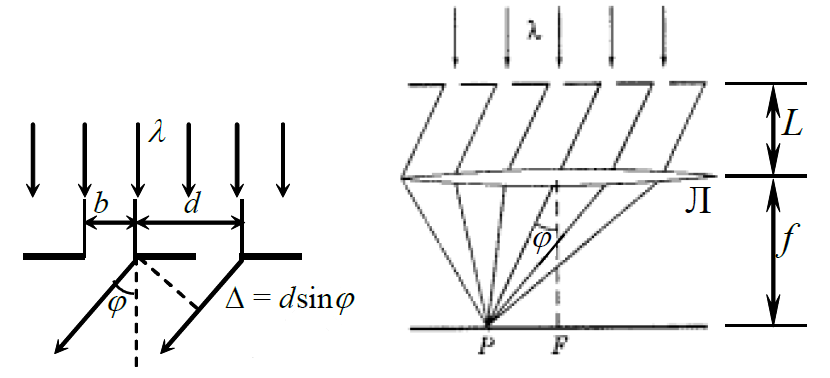
\includegraphics[width=0.5\textwidth]{3.2.png}
        % Підпис (зазвичай під малюнком):
        \caption{}
        % Мітка для посилань у тексті (\ref{fig:...})
        \label{fig2:schema}

    \end{figure}
    
    то розподіл інтенсивності світла описується функцією

    \begin{equation}
        \displaystyle I = I_0 \dfrac{\sin^2 \left( \dfrac{\pi b}{\lambda} \sin \varphi \right)}{\left( \dfrac{\pi b}{\lambda} \sin \varphi \right)^2} \cdot \dfrac{\sin^2 \left( \dfrac{N\pi d}{\lambda} \sin \varphi \right)}{\sin^2 \left( \dfrac{\pi d}{\lambda} \sin \varphi \right)},
        \tag{3.4}
    \end{equation}

    графік якої схематично представлений на рис. 3.3.

    \begin{figure}[!ht]

        \renewcommand{\thefigure}{3.\arabic{figure}} % робимо "3.1", "3.2" і т.д.

        \centering
        % Підставляєте потрібний шлях та розмір зображення:
        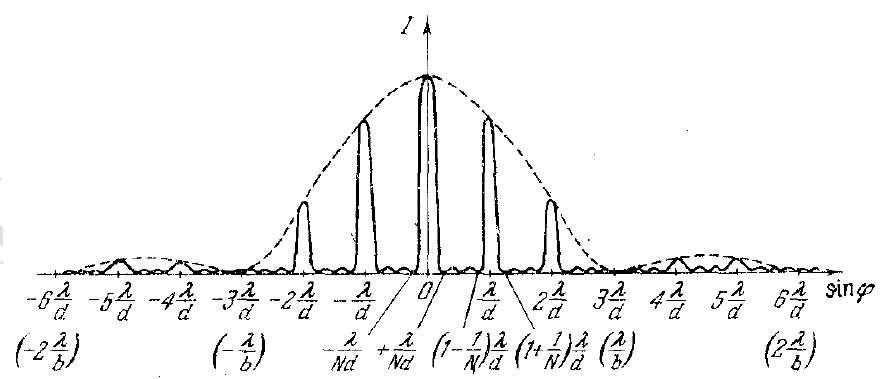
\includegraphics[width=0.5\textwidth]{3.3.png}
        % Підпис (зазвичай під малюнком):
        \caption{}
        % Мітка для посилань у тексті (\ref{fig:...})
        \label{fig3:schema}

    \end{figure}

    Умова спостереження головних максимумів інтенсивності має вигляд

    \begin{equation}
        d \sin \varphi = \pm m\lambda, \quad m = 0, 1, 2, \dots,
        \tag{3.5}
    \end{equation}

    де $d$ – період дифракційної ґратки, який дорівнює сумі ширини прозорої та
    непрозорої частин (див. рис. 3.2).

    \newpage

    \begin{center} \textbf{\Large Практична частина} \end{center}

    \begin{center} \textbf{Опис експериментальної установки та методика вимірювань} \end{center}

    Схема експериментальної установки показана на рис. З.4.

    \begin{figure}[!ht]

        \renewcommand{\thefigure}{3.\arabic{figure}} % робимо "3.1", "3.2" і т.д.

        \centering
        % Підставляєте потрібний шлях та розмір зображення:
        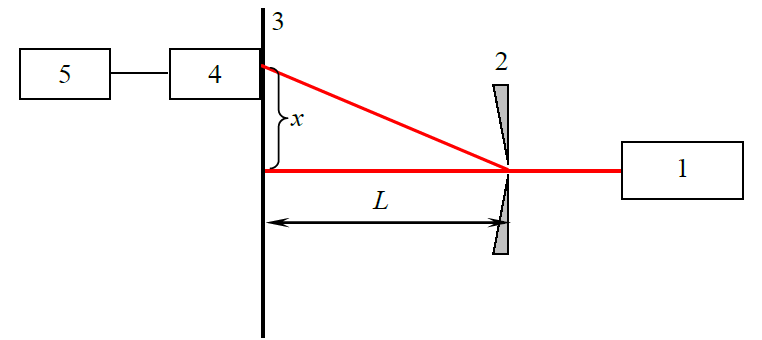
\includegraphics[width=0.5\textwidth]{3.4.png}
        % Підпис (зазвичай під малюнком):
        \caption{}
        % Мітка для посилань у тексті (\ref{fig:...})
        \label{fig4:schema}

    \end{figure}

    Джерелом світла у
    даній роботі є Не-Ne лазер 1, що генерує практично плоску монохроматичну
    хвилю у червоній ділянці спектра. Світлова хвиля направляється на розсувну
    щілину 2 перпендикулярно до її площини. Щілина має мікрогвинт, за допомогою
    якого можна встановлювати потрібну ширину.

    Дифракційна картина спостерігається на екрані 3. У площині екрана можна
    зміщувати фотоприймач 4 з малим вхідним отвором. Сигнал із фотоприймача
    (фотоприймачем є фотодіод), пропорційний середній інтенсивності світла, що
    пройшло крізь вхідний отвір, після підсилення вимірюється вольтметром 5.

    Якщо підібрати ширину щілини 2 так, щоб ширина дифракційного
    максимуму була набагато більшою за розмір вхідного отвору фотоприймача, то за
    допомогою такої експериментальної установки можна достатньо точно виміряти
    розподіл інтенсивності $I(\varphi)$ пучка, що дифрагував і, відповідно, експериментально
    перевірити вираз (3.1).

    Для спостереження дифракії на ґратці її ставлять на місце щілини.

    \textbf{УВАГА!} Категорично забороняється спостерігати світловий пучок, направлений
    безпосередньо від лазера на око або після його відбивання дзеркальною
    поверхнею, тому що це є небезпечним для зору. Лазерний пучок можна
    спостерігати лише розсіяним на не дзеркальних поверхнях (аркуш паперу тощо).

    \begin{center} \textbf{Порядок виконання} \end{center}

    Завдання №1. Дифракція на щілині

    \begin{enumerate}
    \item Увімкнув експериментальну установку згідно з інструкцією.
    \item Встановив щілину у центрі лазерного пучка.
    \item Плавно обертав мікрометричний гвинт до появи дифракційної картини на екрані. Зафіксував мінімальну ширину щілини~$b_{\min}$.
    \item Продовжував збільшувати ширину щілини, спостерігаючи за звуженням дифракційної картини, та зафіксував максимальну ширину~$b_{\max}$, при якій ще видно чітку інтерференційну структуру.
    \item Провів серію вимірювань:
        \begin{itemize}
        \item визначив координати~$X_i$ фотоприймача;
        \item записав покази вольтметра~$U_i$;
        \item зібрав не менше 5 точок у центральному максимумі й по 3 — у кожному побічному.
        \end{itemize}
    \item Обчислив кути дифракції:
        \[
        \varphi_i = \frac{X_i}{L},
        \]
        де $L$ — відстань від щілини до екрана.
    \item Обчислив теоретичні значення відносної інтенсивності $I(\varphi_i)/I_0$ за формулою (3.1) та заніс у таблицю~3.1.
    \item Побудував графіки:
        \begin{itemize}
        \item експериментальної залежності $I/I_0$ від $\varphi$;
        \item теоретичної кривої на основі формули (3.1).
        \end{itemize}
    \item Зробив аналіз графіків: оцінив збіг експерименту з теорією, зазначив можливі відхилення.
    \item За графіком визначив положення максимумів і мінімумів, записав у таблицю~3.3.
    \item Використовуючи умову екстремумів $b\varphi = m\lambda$ і метод найменших квадратів, обчислив:
        \[
        \lambda, \quad \sigma_\lambda.
        \]
    \item Знайшов відношення ширини щілини до довжини хвилі:
        \[
        \frac{b_{\min}}{\lambda}, \quad \frac{b_{\max}}{\lambda}
        \]
        і порівняв з теоретичними межами.
    \end{enumerate}

    Завдання №2. Дифракція на ґратці

    \begin{enumerate}
    \item Замінено щілину на дифракційну ґратку, встановлено її перпендикулярно до лазерного пучка.
    \item Отримано дифракційну картину на екрані.
    \item Виміряно відстані $X_i$ від центра картини до головних максимумів.
    \item Усереднено симетричні значення, результати занесено у таблицю~3.2.
    \item Обчислено кути:
        \[
        \varphi_i = \frac{X_i}{L}
        \]
    \item Обчислено $ \sin \varphi_i $ та внесено у таблицю~3.2.
    \end{enumerate}

    \newpage

    TABLE 2

    \newpage

    \begin{figure}[ht]
        \includegraphics[width=1.0\textwidth]{graph_photo.png}
    \end{figure}

    \renewcommand{\arraystretch}{2.5}  % висота рядків

    \begin{table}[ht]
    \centering
    \medskip
    \begin{tabular}{|*{9}{c|}}  % 13 колонок, усі centered
        \hline
        \multirow{2}{*}{\makecell[c]{Аргумент\\МНК $p$}}
        & \makecell[c]{1-й\\min}
        & \makecell[c]{1-й\\max}
        & \makecell[c]{2-й\\min}
        & \makecell[c]{2-й\\max}
        & \makecell[c]{3-й\\min}
        & \makecell[c]{3-й\\max}
        & \makecell[c]{4-й\\min}
        & \makecell[c]{4-й\\max}
        \\
        \cline{2-9}
        & \makecell[c]{\rule{0pt}{3.5ex}1}
        & \makecell[c]{\rule{0pt}{3.5ex}$1\tfrac{1}{2}$}
        & \makecell[c]{\rule{0pt}{3.5ex}2}
        & \makecell[c]{\rule{0pt}{3.5ex}$2\tfrac{1}{2}$}
        & \makecell[c]{\rule{0pt}{3.5ex}3}
        & \makecell[c]{\rule{0pt}{3.5ex}$3\tfrac{1}{2}$}
        & \makecell[c]{\rule{0pt}{3.5ex}4}
        & \makecell[c]{\rule{0pt}{3.5ex}$4\tfrac{1}{2}$}
        \\
        \hline
        \makecell[c]{$\varphi_i$, рад}
        & 0,0111
        & 0,0133
        & 0,0156
        & 0,0178
        & 0,0200
        & 0,0236
        & 0,0258
        & 0,0289
        \\
        \hline
    \end{tabular}
    \end{table}

    Відповідно для обчислення значення $\lambda$ потрібно використовувати метод найменших квадратів. Для спрощення розрахунків, я застосую
    програмне забезпечення лінійної регресії бібліотеки \texttt{numpy}, а саме \texttt{numpy.polyfit}, який окрім як знаходить коефіцієнти лінійної залежності, так і 
    суми квадратів похибок, з яких я знайду середньоквадратичну похибку.
    Тоді за результатами обчислень, $\lambda \approx 609{,}43$ нм, $\sigma_{\lambda} \approx 50{,}09$ нм.

    Відповідне значення $b_{max}\slash \lambda$, $b_{min} \slash \lambda$ дорівнюють 49{,}23 та 344{,}59 відповідно (за результатми обчислення програми).

    Із періодом дифракційної гратки та його середньоквадратичною похибкою зроблю так само. За результатами виконання програми, отримую:
    $d \approx 1723{,}01$ мкм, $\sigma_d \approx 1{,}57$ мкм.

    Звідси при $q = 13$ видимих максимумів

    \vspace{5pt}
    
    $\displaystyle b = \frac{d}{q} = \frac{1723{,}01 \cdot 10^{-6}}{13} \approx 132{,}54$ мкм, що є досить близьким значенням до реального значення $b$.

    \newpage

    \setlength{\parindent}{0pt}

    Результат виконання програми:

    \begin{figure}[ht]
        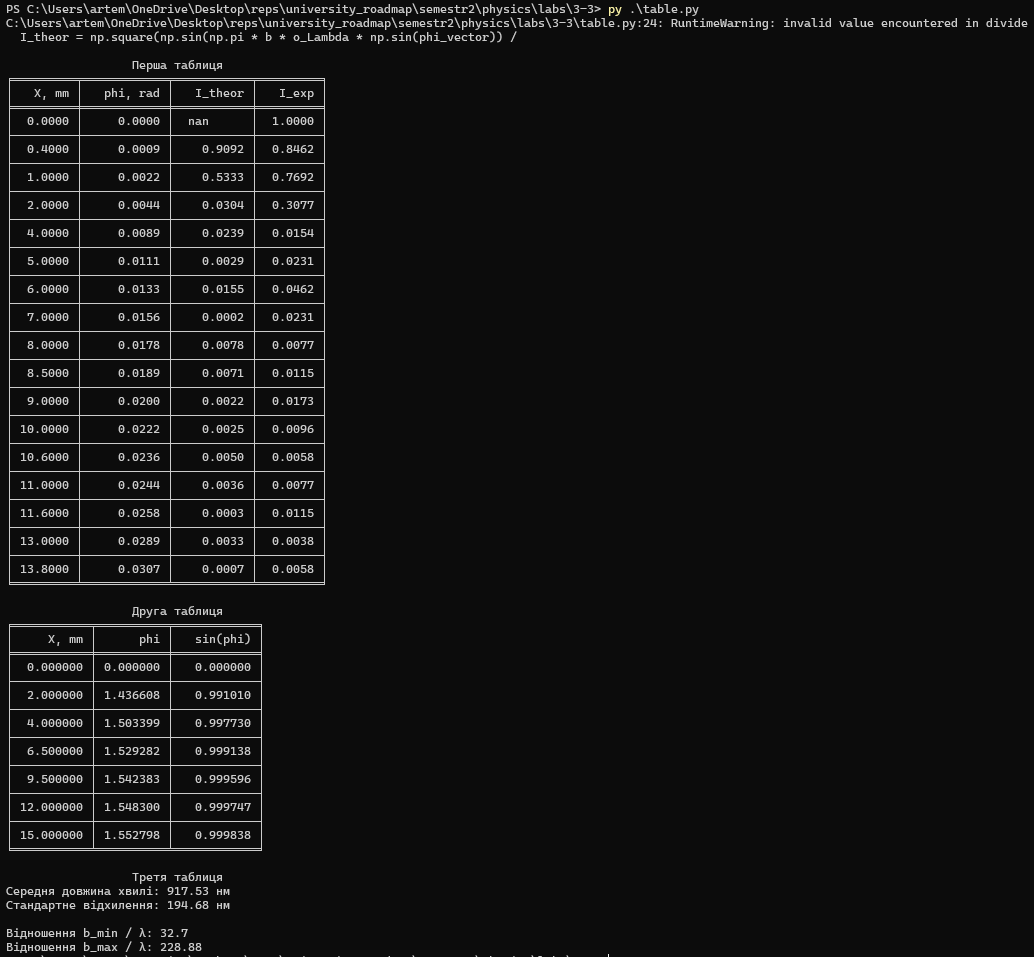
\includegraphics[width=0.9\textwidth]{programm_running.png}
    \end{figure}

    \newpage

    \textbf{Висновок:}

    У ході лабораторної роботи досліджено дифракцію Фраунгофера на щілині та дифракційній ґратці. Експериментально підтверджено залежність інтенсивності світла від кута дифракції, передбачену теоретичними формулами. За результатами обробки експериментальних даних визначено довжину хвилі лазерного випромінювання:
    \[
    \lambda = 609{,}43\,\text{нм},\quad \sigma_{\lambda} = 50{,}09\,\text{нм}.
    \]
    Розраховані значення ширини щілини відносно довжини хвилі:
    \[
    \frac{b_{\min}}{\lambda} \approx 49{,}23,\quad \frac{b_{\max}}{\lambda} \approx 344{,}59,
    \]
    що відповідає умовам виникнення чіткої дифракційної картини. Таким чином, експериментальні результати добре узгоджуються з теоретичними перед­баченнями, підтверджуючи справедливість закону дифракції Фраунгофера.







\begin{center} \textbf{\large Контрольні питання} \end{center}

\begin{enumerate}
  \item \textit{Що таке дифракція світла?} \\
  Дифракція --- це огинання світловими хвилями перешкод або проходження через вузькі отвори, внаслідок чого виникає характерне інтерференційне розподілення інтенсивності.

  \item \textit{Чи існує принципова відмінність між дифракцією та інтерференцією?} \\
  Обидва явища базуються на когерентному накладанні хвиль. Принципова відмінність: інтерференція — це результат накладання декількох хвиль від різних джерел, а дифракція — результат самоналоження хвилі після огинання перешкоди.

  \item \textit{Принцип Гюйгенса–Френеля та аналітичний вираз:} \\
  Кожна точка фронту хвилі є джерелом вторинних хвиль. Новий фронт — огинаюча всіх вторинних хвиль. \\ 
  Аналітичний вираз: 
  \[
    E(P) = \frac{1}{i\lambda} \iint_S E(Q) \frac{e^{ikr}}{r} K(\theta)\, dS
  \]
  де $K(\theta)$ — коефіцієнт напрямленості, $r$ — відстань між точками $Q$ та $P$.

  \item \textit{Чим відрізняється дифракція Фраунгофера від дифракції Френеля?} \\
  У дифракції Френеля джерело й екран на скінченній відстані. У Фраунгофера — на нескінченності (або колімоване світло), хвильові фронти — плоскі.

  \item \textit{Де локалізована картина Фраунгофера з лінзою та без?} \\
  \begin{itemize}
    \item Без лінзи — на нескінченності.
    \item З лінзою — у фокальній площині збиральної лінзи.
  \end{itemize}

  \item \textit{Залежність інтенсивності дифракції на щілині:} \\
  \[
    I(\varphi) = I_0 \left( \frac{\sin(\beta)}{\beta} \right)^2,
    \quad \text{де } \beta = \frac{\pi b \sin \varphi}{\lambda}
  \]
  Графік має центральний максимум і симетричні менші побічні.

  \item \textit{Умови максимумів та мінімумів:} \\
  Для щілини:
  \[
    b \sin\varphi = m\lambda \Rightarrow \text{мінімуми}
  \]
  Для ґратки:
  \[
    d \sin\varphi = m\lambda \Rightarrow \text{максимуми}
  \]

  \item \textit{Межі для ширини щілини:} \\
  Для спостереження: \( \lambda \leq b \leq 10^3\lambda \). Зі зростанням $b$ — картина звужується, центральний максимум стискається.

  \item \textit{Критерії Френеля, Фраунгофера, геометричної оптики:} \\
  \begin{itemize}
    \item Френеля: $z \sim D^2/\lambda$
    \item Фраунгофера: $z \gg D^2/\lambda$
    \item Геометрична оптика: $\lambda \rightarrow 0$
  \end{itemize}
  Тлумачення — порівняння з розмірами зон Френеля.

  \item \textit{Що буде при закритті половини лінзи?} \\
  Інтенсивність зменшиться, але структура дифракційної картини залишиться незмінною.

  \item \textit{Відношення інтенсивностей побічних максимумів:} \\
  Для однієї щілини:
  \[
    \frac{I_m}{I_0} = \left( \frac{\sin(\pi m)}{\pi m} \right)^2
  \]
  Наприклад, для $m = 1$: $\approx 4.5\%$ від $I_0$.

  \item \textit{Зсув щілини паралельно фокальній площині:} \\
  Картина не зміниться за формою, але зміститься у площині екрана.

  \item \textit{Число головних максимумів ґратки:} \\
  Залежить від співвідношення $d/\lambda$ та числа щілин $N$:
  \[
    m_{\text{max}} \leq \frac{d}{\lambda}
  \]

  \item \textit{Відношення ширин максимуму ґратки і мінімуму щілини:} \\
  \[
    \frac{\Delta\theta_{\text{ґратки}}}{\Delta\theta_{\text{щілини}}} = \frac{b}{Nd}
  \]

  \item \textit{Підсилення інтенсивності головного максимуму ґратки:} \\
  В $N^2$ разів сильніше, ніж для однієї щілини. Інтенсивність:
  \[
    I \sim E^2 \sim N^2
  \]
  \textit{Інтенсивність} — це середнє значення потоку енергії, пропорційне квадрату амплітуди хвилі.

  \item \textit{Вимірювання інтенсивності:} \\
  В роботі використано фотодіод, що перетворює світловий потік в електричний сигнал. Вольтметр реєструє напругу, пропорційну інтенсивності світла: $I \sim U$.
\end{enumerate}

    \vspace{3em}

    \textbf{\large Код програми:}

    \vspace{1em}

    \small{ 

\begin{verbatim}
import numpy as np
from tabulate import tabulate

# CONSTANTS
L = 450e-3  # Відстань від щілини до екрана (в метрах)
b = 0.12e-3  # Ширина щілини (в метрах)
b_min = 0.03e-3  # Мінімальна ширина щілини (в метрах)
b_max = 0.21e-3  # Максимальна ширина щілини (в метрах)
Lambda = 0.63e-6  # Довжина хвилі лазера (в метрах)
o_Lambda = 1 / Lambda  # Обернена довжина хвилі (1/метр)

# First Table

# Масив координат фотоприймача (в міліметрах)
X_vector = np.array([0, 0.4, 1, 2, 4, 5, 6, 7, 8, 8.5,
9, 10, 10.6, 11, 11.6, 13, 13.8])

# Масив показів вольтметра (в поділках)
U_vector = np.array([2600, 2200, 2000, 800, 40, 60, 120,
60, 20, 30, 45, 25, 15, 20, 30, 10, 15])

# Обчислення кутів дифракції (в радіанах)
phi_vector = X_vector * 1e-3 / L  # Переводимо X в метри та
ділимо на L

# Теоретичні значення відносної інтенсивності (формула дифракції)
I_theor = np.square(np.sin(np.pi * b * o_Lambda * np.sin(phi_vector)) / 
                    (np.pi * b * o_Lambda * np.sin(phi_vector)))

# Експериментальні значення відносної інтенсивності
I_exp = U_vector / 2600  # Нормалізація на максимальне значення

# Виведення першої таблиці
print(f"\n{'Перша таблиця':^50}")
print(tabulate(
    np.array([X_vector, phi_vector, I_theor, I_exp]).T,  #
    Транспонування для табличного вигляду
    headers=["X, mm", "phi, rad", "I_theor", "I_exp"],  #
    Заголовки стовпців
    tablefmt="fancy_grid",  # Формат таблиці
    floatfmt=".4f",  # Формат чисел (4 знаки після коми)
))

# Second Table

# Новий масив координат фотоприймача (в міліметрах)
X_vector = np.array([0, 2, 4, 6.5, 9.5, 12, 15])

# Нова відстань від щілини до екрана (в метрах)
L = 270e-3

# Обчислення sin(phi) для кожного X
sin_vector = X_vector / np.sqrt(X_vector**2 + L**2)

# Обчислення кутів phi (в радіанах) через arcsin
phi_vector = np.arcsin(sin_vector)

# Виведення другої таблиці
print(f"\n{'Друга таблиця':^50}")
print(tabulate(
    np.array([X_vector, phi_vector, sin_vector]).T,  #
    Транспонування для табличного вигляду
    headers=["X, mm", "phi", "sin(phi)"],  # Заголовки стовпців
    tablefmt="fancy_grid",  # Формат таблиці
    floatfmt=".6f",  # Формат чисел (6 знаків після коми)
))

# Third Table Work

# Масив кутів phi (в радіанах) для третьої таблиці
phi_vector = np.array([0.0111, 0.0133, 0.0156, 0.0178, 0.0200,
0.0236, 0.0258, 0.0289])

# Масив порядкових номерів максимумів (m)
m_vector = np.array([1, 1.5, 2, 2.5, 3, 3.5, 4, 4.5])

# Лінійна апроксимація залежності phi*b від m
(lambda_var, intercept), residuals, *_ = np.polyfit(m_vector,
phi_vector * b, 1, full=True)

# Обчислення залишкової суми квадратів
residual_sum_of_squares = residuals[0]

# Обчислення середньоквадратичної похибки (RMSE)
rmse = np.sqrt(residual_sum_of_squares / len(phi_vector))

# Виведення результатів для довжини хвилі
print(f"\nlambda: {lambda_var*1e9:.2f} нм")  # Довжина хвилі в наноме
трах
print(f"delta lambda = {rmse*1e9:.2f} нм")  # Похибка довжини хвилі в
нанометрах

# Обчислення відношення мінімальної ширини щілини до довжини хвилі
print(f"\nВідношення b_min / lambda: {round(b_min / lambda_var, 2)}")

# Обчислення відношення максимальної ширини щілини до довжини хвилі
print(f"Відношення b_max / lambda: {round(b_max / lambda_var, 2)}")

# Масив значень sin(phi) для четвертої таблиці
sin_vector = np.array([0, 0.991010, 0.997730, 0.999138, 0.999596,
0.999747, 0.999838])

# Масив порядкових номерів максимумів (m)
m_vector = np.array([0, 1, 2, 3, 4, 5, 6])

# Лінійна апроксимація залежності m від sin(phi)
(coef, intercept), residuals, *_ = np.polyfit(sin_vector, m_vector,
1, full=True)

# Обчислення залишкової суми квадратів
residual_sum_of_squares = residuals[0]

# Обчислення середньоквадратичної похибки (RMSE)
rmse = np.sqrt(residual_sum_of_squares / len(sin_vector))

# Виведення результатів для періоду решітки
print(f"\nd: {lambda_var/coef*1e10:.2f} мкм")  # Період решітки в
мікрометрах
print(f"delta d = {rmse:.2f} мкм")  # Похибка періоду решітки в
мікрометрах
\end{verbatim}
}




\end{document}